% ============================================================
%  Fixed-Wing UAV for Emergency Medical Delivery
%  AS5213: Conceptual Design of UAVs — Group 11: Skunk Works
%  Optimized Beamer Presentation
% ============================================================
\documentclass[aspectratio=169,11pt]{beamer}

% ---------- Core Packages ----------
\usepackage{tikz}
\usetikzlibrary{positioning, arrows.meta, shapes.geometric,
                shadows.blur, decorations.pathmorphing}
\usepackage{pgfplots}
\pgfplotsset{compat=1.18}
\usepackage{booktabs}
\usepackage{amsmath}
\usepackage{siunitx}
\usepackage{graphicx}
\usepackage{array}
\usepackage{multirow}
\usepackage{xcolor}
\usepackage{caption}
\captionsetup{font=scriptsize, labelformat=empty, skip=2pt}

% ---------- Colour Palette (Aerospace) ----------
\definecolor{navydeep}{RGB}{6,90,130}
\definecolor{navymain}{RGB}{28,114,147}
\definecolor{tealaccent}{RGB}{33,41,92}
\definecolor{lightblue}{RGB}{202,220,252}
\definecolor{iceblue}{RGB}{232,243,255}
\definecolor{warmgray}{RGB}{100,100,100}
\definecolor{successgreen}{RGB}{0,128,64}

% ---------- Theme ----------
\usetheme{Madrid}
\usecolortheme{default}
\setbeamertemplate{navigation symbols}{}

% Custom footline: group name left, slide number right
\setbeamertemplate{footline}{%
  \leavevmode%
  \hbox{%
    \begin{beamercolorbox}[wd=.5\paperwidth,ht=2.25ex,dp=1ex,leftskip=1em]{palette primary}%
      \usebeamerfont{author in head/foot}\textbf{Group 11: Skunk Works}%
    \end{beamercolorbox}%
    \begin{beamercolorbox}[wd=.5\paperwidth,ht=2.25ex,dp=1ex,rightskip=1em,right]{palette secondary}%
      \usebeamerfont{date in head/foot}%
      \insertshortdate{}\hspace{2em}\insertframenumber{} / \inserttotalframenumber%
    \end{beamercolorbox}}%
}

% Colour assignments
\setbeamercolor{palette primary}    {bg=navydeep,  fg=white}
\setbeamercolor{palette secondary}  {bg=navymain,  fg=white}
\setbeamercolor{palette tertiary}   {bg=tealaccent,fg=white}
\setbeamercolor{palette quaternary} {bg=navymain,  fg=white}
\setbeamercolor{structure}          {fg=navydeep}
\setbeamercolor{section in toc}     {fg=navymain}
\setbeamercolor{frametitle}         {bg=navymain,  fg=white}
\setbeamercolor{title}              {fg=white}
\setbeamercolor{block title}        {bg=navymain,  fg=white}
\setbeamercolor{block body}         {bg=iceblue,   fg=black}
\setbeamercolor{alerted text}       {fg=navydeep}
\setbeamercolor{itemize item}       {fg=navymain}
\setbeamercolor{itemize subitem}    {fg=navymain}

% Bullet style
\setbeamertemplate{itemize items}[circle]
\setbeamertemplate{enumerate items}[circle]

% Slightly tighter frametitle
\setbeamertemplate{frametitle}{%
  \vspace{0.15em}
  \insertframetitle
}

% ---------- Document Metadata ----------
\title{\textbf{Fixed-Wing UAV for Emergency Medical Delivery}}
\subtitle{AS5213: Conceptual Design of UAVs}
\author{DS Vivek \and Divyam Pandey \and G. Vishwas \and
        Manav Agarwal \and Monisha V \and Abhijeet Mangela}
\institute{Group 11: Skunk Works \\ Department of Aerospace Engineering \\ IIT Madras}
\date{April 2026}

% ---------- Convenience command for highlighted specs ----------
\newcommand{\spec}[1]{\textcolor{navydeep}{\textbf{#1}}}

% ============================================================
\begin{document}

% ========== SLIDE 1 — TITLE ==========
{
\setbeamertemplate{footline}{}
\setbeamercolor{background canvas}{bg=navydeep}
\begin{frame}[noframenumbering]
  \titlepage
  \vspace{-0.4cm}
  \begin{center}
    \colorbox{white!90!navydeep}{%
      \parbox{0.72\textwidth}{%
        \centering
        \vspace{3pt}
        \textcolor{navymain}{\small\textbf{[IMAGE PLACEHOLDER: Isometric CAD render]}}
        \vspace{3pt}
      }%
    }
  \end{center}
\end{frame}
}

% ========== SLIDE 2 — MISSION REQUIREMENTS ==========
\begin{frame}{Mission Profile \& Requirements (1/2)}

\begin{columns}[T]

  \column{0.52\textwidth}
  \begin{block}{Design Objective}
    Fixed-wing UAV for \textbf{time-critical medical delivery} of
    antivenom and blood products to remote / underserved areas.
  \end{block}

  \vspace{0.35cm}
  \textbf{\color{navymain}Key Performance Requirements:}
  \begin{itemize}
    \item Operational radius: \spec{\SIrange{40}{50}{\kilo\meter}}
    \item Total range: \spec{\SIrange{80}{100}{\kilo\meter}}
    \item Cruise speed: \spec{\SIrange{18}{25}{\meter\per\second}}
    \item STOL takeoff distance: \spec{$<\SI{150}{\meter}$}
    \item Endurance: \spec{\SIrange{1}{2}{\hour}}
  \end{itemize}

  \column{0.46\textwidth}
  \begin{block}{Design Constraints}
    \begin{itemize}
      \item Max wingspan: \spec{\SI{2.00}{\meter}}
      \item Payload capacity: \spec{\SI{1.00}{\kilo\gram}} (droppable)
      \item Electric propulsion
      \item Autonomous \& BVLOS capable
    \end{itemize}
  \end{block}

  \vspace{0.3cm}
  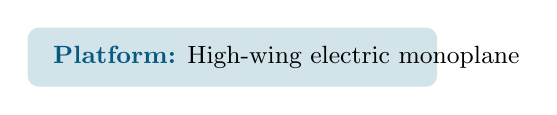
\begin{tikzpicture}
    \fill[navymain!20, rounded corners=4pt] (0,0) rectangle (5.2,0.75);
    \node[anchor=west, font=\small] at (0.2,0.375)
      {\textbf{\color{navydeep}Platform:} High-wing electric monoplane};
  \end{tikzpicture}

\end{columns}
\end{frame}

% ========== SLIDE 3 — MISSION PROFILE ==========
\begin{frame}{Mission Profile \& Requirements (2/2)}

\begin{columns}[T]

  \column{0.38\textwidth}
  \textbf{\color{navymain}Mission Phases:}
  \begin{enumerate}\setlength\itemsep{3pt}
    \item Takeoff (STOL, $<\SI{150}{\meter}$)
    \item Climb to cruise altitude
    \item Cruise — outbound leg
    \item \spec{Payload airdrop} (no landing)
    \item Turn / loiter
    \item \spec{Re-climb phase}
    \item Cruise — inbound leg
    \item Descent \& landing
  \end{enumerate}

  \column{0.60\textwidth}
  \begin{figure}
    \centering
    \includegraphics[width=\linewidth, height=0.62\textheight, keepaspectratio]%
      {Mission_Profile_new.png}
    \caption{UAV Mission Profile Diagram}
  \end{figure}

\end{columns}
\end{frame}

% ========== SLIDE 4 — DESIGN METHODOLOGY ==========
\begin{frame}{Design Methodology}
\vspace{-0.2cm}
\begin{center}
\resizebox{0.93\textwidth}{!}{%
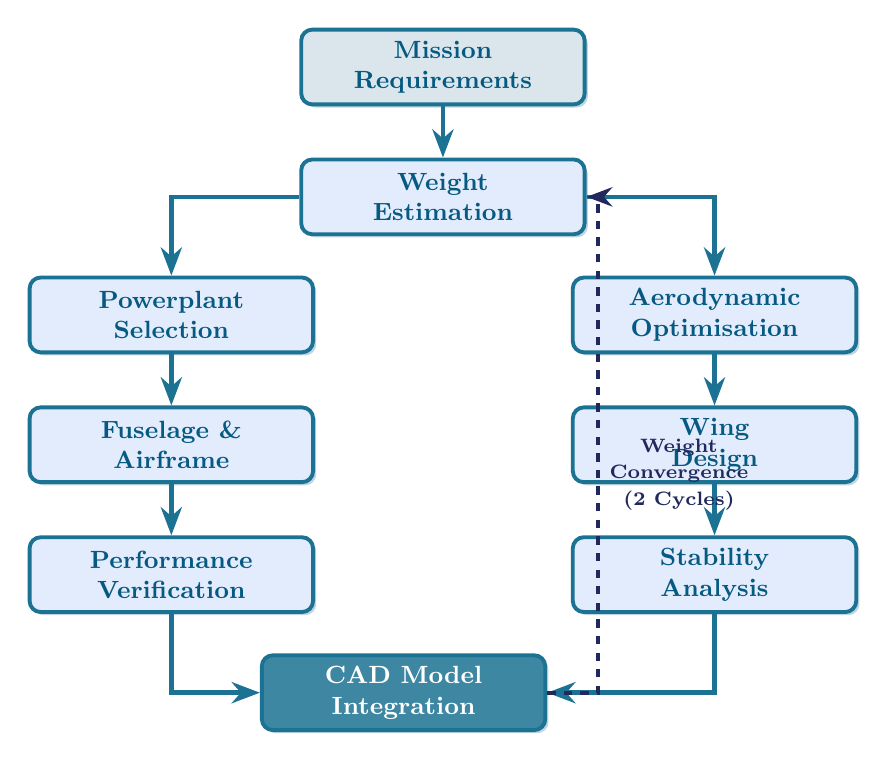
\begin{tikzpicture}[
  node distance=0.65cm and 1.1cm,
  box/.style={
    rectangle, draw=navymain, rounded corners=4pt, line width=1.4pt,
    minimum width=3.6cm, minimum height=0.95cm, align=center,
    fill=white,
    drop shadow={shadow xshift=0.4mm,shadow yshift=-0.4mm,opacity=0.25,fill=navydeep},
    font=\fontsize{9}{11}\selectfont\bfseries
  },
  boxstart/.style ={box, fill=navydeep!15, text=navydeep},
  boxproc/.style  ={box, fill=lightblue!55, text=navydeep},
  boxend/.style   ={box, fill=navymain!85, text=white},
  arrow/.style    ={->, line width=1.6pt, >=Stealth, color=navymain},
  arrowback/.style={->, line width=1.4pt, >=Stealth, color=tealaccent, dashed}
]
  \node[boxstart] (req)  {Mission\\Requirements};
  \node[boxproc,  below=of req]                    (wt)   {Weight\\Estimation};
  \node[boxproc,  below left=0.5cm and -0.2cm of wt]  (pwr)  {Powerplant\\Selection};
  \node[boxproc,  below right=0.5cm and -0.2cm of wt] (aero) {Aerodynamic\\Optimisation};
  \node[boxproc,  below=of pwr]                    (fuse) {Fuselage \&\\Airframe};
  \node[boxproc,  below=of aero]                   (wing) {Wing\\Design};
  \node[boxproc,  below=of fuse]                   (perf) {Performance\\Verification};
  \node[boxproc,  below=of wing]                   (stab) {Stability\\Analysis};
  \node[boxend,   below right=0.5cm and -0.7cm of perf] (cad)  {CAD Model\\Integration};

  \draw[arrow] (req)  -- (wt);
  \draw[arrow] (wt)   -| (pwr);
  \draw[arrow] (wt)   -| (aero);
  \draw[arrow] (pwr)  -- (fuse);
  \draw[arrow] (aero) -- (wing);
  \draw[arrow] (fuse) -- (perf);
  \draw[arrow] (wing) -- (stab);
  \draw[arrow] (perf) |- (cad);
  \draw[arrow] (stab) |- (cad);

  \draw[arrowback] (cad.east) -- ++(0.65,0) |-
    node[pos=0.22, right, align=center, font=\fontsize{7.5}{9.5}\selectfont\bfseries, text=tealaccent]
      {Weight\\Convergence\\(2 Cycles)}
    (wt.east);
\end{tikzpicture}%
}
\end{center}
\end{frame}

% ========== SLIDE 5 — POWERPLANT (1/2) ==========
\begin{frame}{Powerplant Specifications (1/2)}

\begin{columns}[T]

  \column{0.48\textwidth}
  \begin{center}
    % T-Motor image not supplied — placeholder kept
    \colorbox{iceblue}{\parbox{0.9\linewidth}{%
      \centering\vspace{6pt}
      \textcolor{navymain}{\small\textbf{[IMAGE: T-Motor AM480 900KV]}}
      \vspace{6pt}
    }}
  \end{center}
  \vspace{0.2cm}
  \textbf{\color{navymain}Motor — T-Motor AM480 900KV:}
  \begin{itemize}\setlength\itemsep{2pt}
    \item Configuration: \spec{Dual-motor tractor}
    \item Max power: \spec{\SI{450}{\watt}} at 80\% throttle
    \item Voltage: \SI{11.1}{\volt} (3S LiPo per motor)
    \item Peak current: \SI{26}{\ampere}
    \item ESC: Hobbywing Skywalker 50A V2
  \end{itemize}

  \column{0.50\textwidth}
  \begin{figure}
    \centering
    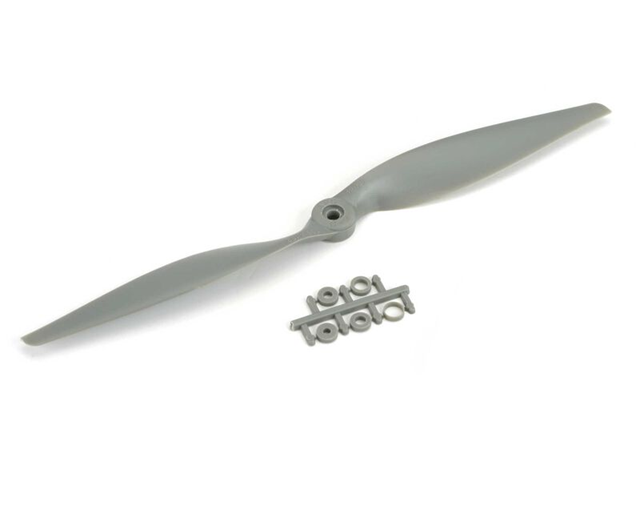
\includegraphics[width=0.72\linewidth, height=0.30\textheight, keepaspectratio]{prp.png}
    \caption{APC 12$\times$6E Propeller}
  \end{figure}
  \vspace{0.1cm}
  \textbf{\color{navymain}Propeller — APC 12$\times$6E:}
  \begin{itemize}\setlength\itemsep{2pt}
    \item Diameter: 12~in (\SI{0.305}{\meter})
    \item Pitch: 6~in
    \item Optimised for \SIrange{300}{350}{\watt} cruise
  \end{itemize}

  \vspace{0.3cm}
  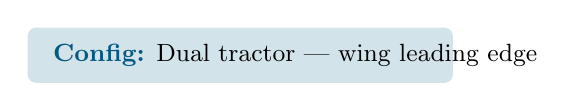
\begin{tikzpicture}
    \fill[navymain!20, rounded corners=3pt] (0,0) rectangle (5.4,0.7);
    \node[anchor=west, font=\small] at (0.2,0.35)
      {\textbf{\color{navydeep}Config:} Dual tractor — wing leading edge};
  \end{tikzpicture}

\end{columns}
\end{frame}

% ========== SLIDE 6 — POWERPLANT (2/2) ==========
\begin{frame}{Powerplant Specifications (2/2)}

\begin{columns}[T]

  \column{0.50\textwidth}
  \begin{figure}
    \centering
    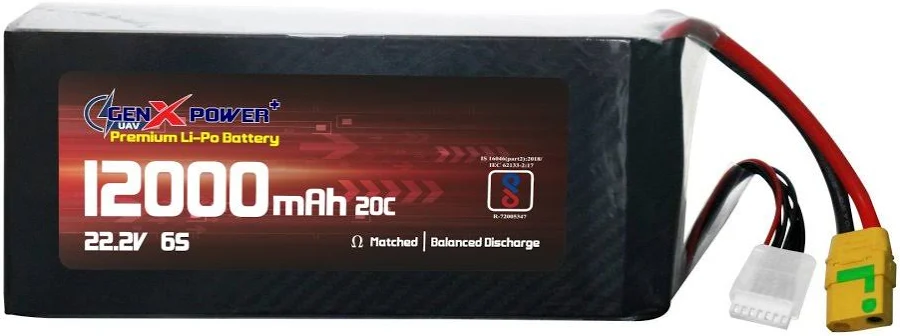
\includegraphics[width=0.80\linewidth, height=0.30\textheight, keepaspectratio]{genx_battery.png}
    \caption{GenX Power+ 6S 12\,000\,mAh LiPo}
  \end{figure}
  \vspace{0.1cm}
  \textbf{\color{navymain}Battery — GenX 6S \SI{12}{\ampere\hour}:}
  \begin{itemize}\setlength\itemsep{2pt}
    \item Voltage: \spec{\SI{22.2}{\volt}} nominal
    \item Capacity: \SI{12000}{\milli\ampere\hour}
    \item Mass: \spec{\SI{1524}{\gram}}
    \item Dimensions: $183\times75\times34$\,mm
    \item Total energy: \SI{959}{\kilo\joule}
  \end{itemize}

  \column{0.48\textwidth}
  \textbf{\color{navymain}Power Budget:}

  \vspace{0.2cm}
  \begin{tabular}{@{}lc@{}}
    \toprule
    \textbf{Item} & \textbf{Value} \\
    \midrule
    Peak power (climb)    & \spec{\SI{361.46}{\watt}} \\
    Required thrust       & \SI{14.73}{\newton} \\
    Avionics load         & \SI{6.61}{\watt} \\
    Battery efficiency    & \spec{85\%} \\
    Motor efficiency      & \spec{82\%} \\
    \bottomrule
  \end{tabular}

  \vspace{0.4cm}
  \begin{block}{Endurance Estimate}
    \centering
    \spec{$\approx$ 2 h 5 min} at cruise power
    (\SI{75}{\watt} avg.)
  \end{block}

\end{columns}
\end{frame}

% ========== SLIDE 7 — AERODYNAMICS (1/2) ==========
\begin{frame}{Aerodynamic Parameters (1/2)}

\begin{columns}[T]

  \column{0.46\textwidth}
  \textbf{\color{navymain}Wing Configuration:}
  \begin{itemize}\setlength\itemsep{3pt}
    \item Airfoil: \spec{Selig S7055}
    \item Planform: Rectangular, high-wing
    \item Aspect ratio $(AR)$: \spec{7.53}
    \item Wing area $(S)$: \SI{0.5307}{\meter\squared}
    \item Wingspan $(b)$: \spec{\SI{2.00}{\meter}}
    \item Mean chord $(\bar{c})$: \SI{0.2653}{\meter}
    \item Taper ratio: 1.0 (rectangular)
  \end{itemize}

  \vspace{0.3cm}
  \textbf{\color{navymain}Drag Polar:}
  \begin{itemize}\setlength\itemsep{2pt}
    \item $C_{D_0} = 0.02873$
    \item Oswald efficiency: $e = 0.85$
    \item $k = \frac{1}{\pi e \cdot AR}$
  \end{itemize}

  \vspace{0.3cm}
  
\begin{tikzpicture}
    \fill[navydeep, rounded corners=3pt] (0,0) rectangle (4.6,1.1);
    \node[text=white, align=center] at (2.3,0.55)
      {\textbf{Max L/D Ratio} \quad \Large\textbf{12.55}};
  \end{tikzpicture}

  \column{0.52\textwidth}
  \begin{figure}
    \centering
    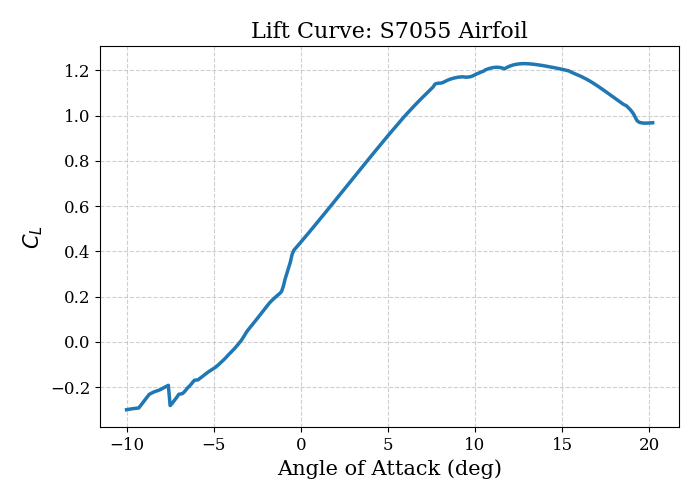
\includegraphics[width=\linewidth, height=0.72\textheight, keepaspectratio]{cl_alp.png}
    \caption{Lift Curve — Selig S7055 Airfoil}
  \end{figure}

\end{columns}
\end{frame}

% ========== SLIDE 8 — AERODYNAMICS (2/2) ==========
\begin{frame}{Aerodynamic Parameters (2/2)}

\begin{columns}[T]

  \column{0.38\textwidth}
  \textbf{\color{navymain}Lift Characteristics:}
  \begin{itemize}\setlength\itemsep{3pt}
    \item $C_{L,\text{cruise}}$: \spec{0.65 – 0.75}
    \item $C_{L,\text{max}}$: \spec{1.40}
    \item Lift-curve slope: $C_{L_\alpha}=\SI{5.73}{\per\radian}$
    \item Stall speed: \spec{\SI{12.4}{\meter\per\second}}
    \item Best L/D at $\alpha \approx 5^\circ$
  \end{itemize}

  \vspace{0.4cm}
  \begin{block}{Key Takeaway}
    Peak $C_L/C_D \approx \mathbf{90}$ for the bare\\
    airfoil; \textbf{12.55} for the full aircraft.
  \end{block}

  \column{0.60\textwidth}
  \begin{figure}
    \centering
    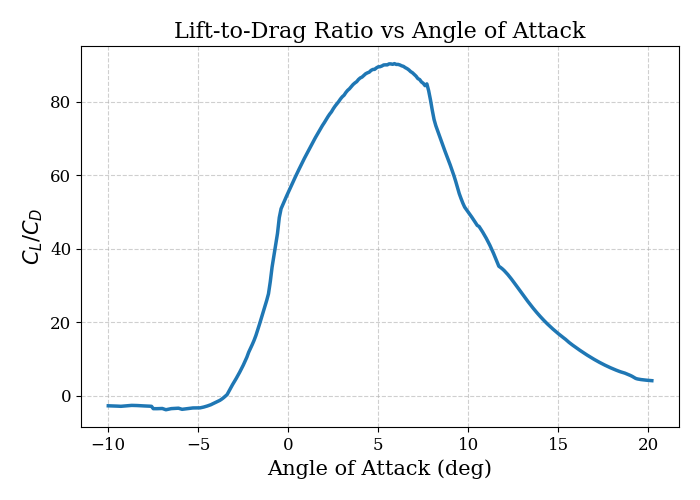
\includegraphics[width=\linewidth, height=0.72\textheight, keepaspectratio]{CL_Cd_alpha.png}
    \caption{Lift-to-Drag Ratio vs. Angle of Attack}
  \end{figure}

\end{columns}
\end{frame}

% ========== SLIDE 9 — INERTIA & GEOMETRY (1/2) ==========
\begin{frame}{Inertia \& Geometric Parameters (1/2)}

\begin{columns}[T]

  \column{0.50\textwidth}
  \textbf{\color{navymain}Mass Breakdown:}

  \vspace{0.2cm}
  \begin{tabular}{@{}lc@{}}
    \toprule
    \textbf{Component} & \textbf{Mass (kg)} \\
    \midrule
    Empty structure     & 3.29  \\
    Battery             & 0.987 \\
    Avionics            & 0.90  \\
    Payload (droppable) & \spec{1.20} \\
    \midrule
    \textbf{MTOW}       & \spec{6.59} \\
    \bottomrule
  \end{tabular}

  \vspace{0.35cm}
  \textbf{\color{navymain}Weight Fractions:}
  \begin{itemize}
    \item Empty weight fraction: 0.50
    \item Payload fraction: 0.18
  \end{itemize}

  \column{0.48\textwidth}
  \textbf{\color{navymain}Centre of Gravity:}

  \vspace{0.2cm}
  \begin{tabular}{@{}lc@{}}
    \toprule
    \textbf{Parameter} & \textbf{Value} \\
    \midrule
    Longitudinal CG  & \SI{264}{\milli\meter} from nose \\
    Neutral point     & \SI{296}{\milli\meter} from nose \\
    Lateral CG        & \SI{0}{\milli\meter} (symmetric) \\
    Static margin     & \spec{$\approx 14\%$ MAC} \\
    \bottomrule
  \end{tabular}

  \vspace{0.4cm}
  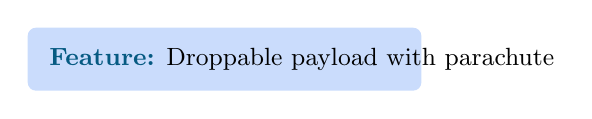
\begin{tikzpicture}
    \fill[lightblue, rounded corners=3pt] (0,0) rectangle (5.0,0.8);
    \node[anchor=west, font=\small] at (0.15,0.4)
      {\textbf{\color{navydeep}Feature:} Droppable payload with parachute};
  \end{tikzpicture}

\end{columns}
\end{frame}

% ========== SLIDE 10 — INERTIA & GEOMETRY (2/2) ==========
\begin{frame}{Inertia \& Geometric Parameters (2/2)}

\begin{columns}[T]

  \column{0.50\textwidth}
  \textbf{\color{navymain}Fuselage Dimensions:}

  \vspace{0.2cm}
  \begin{tabular}{@{}lc@{}}
    \toprule
    \textbf{Parameter} & \textbf{Value} \\
    \midrule
    Total length          & \SI{1.10}{\meter} \\
    Fuselage diameter     & \SI{0.15}{\meter} \\
    Tail boom length      & \SI{0.70}{\meter} \\
    \bottomrule
  \end{tabular}

  \vspace{0.4cm}
  \textbf{\color{navymain}Control Surfaces:}
  \begin{itemize}\setlength\itemsep{2pt}
    \item Elevator, rudder, ailerons (4 servos)
    \item Elevator deflection: $-15^\circ$ to $+25^\circ$
  \end{itemize}

  \column{0.48\textwidth}
  \textbf{\color{navymain}Empennage:}

  \vspace{0.2cm}
  \begin{tabular}{@{}lc@{}}
    \toprule
    \textbf{Parameter} & \textbf{Value} \\
    \midrule
    H-tail area ($S_t$)    & \SI{0.133}{\meter\squared} \\
    H-tail span            & \SI{0.773}{\meter} \\
    Tail arm ($l_t$)       & \SI{0.70}{\meter} \\
    H-tail airfoil         & NACA 0012 \\
    Setting angle ($i_t$)  & $-0.31^\circ$ \\
    V-tail area ($S_v$)    & \SI{0.080}{\meter\squared} \\
    \bottomrule
  \end{tabular}

\end{columns}
\end{frame}

% ========== SLIDE 11 — PERFORMANCE (1/2) ==========
\begin{frame}{Performance Parameters (1/2)}

\begin{columns}[T]

  \column{0.42\textwidth}
  \textbf{\color{navymain}Flight Envelope Summary:}

  \vspace{0.15cm}
  \begin{tabular}{@{}lc@{}}
    \toprule
    \textbf{Parameter} & \textbf{Value} \\
    \midrule
    Max range       & \spec{\SI{83.15}{\kilo\meter}} \\
    Endurance       & \spec{2\,h\,5\,min} \\
    Cruise speed    & \spec{\SIrange{18}{22}{\meter\per\second}} \\
    Stall speed     & \SI{12.4}{\meter\per\second} \\
    Max speed       & \SI{28}{\meter\per\second} \\
    Service ceiling & \SI{2000}{\meter} \\
    \midrule
    Rate of climb   & \spec{\SI{3.5}{\meter\per\second}} \\
    Climb angle     & $15^\circ$–$20^\circ$ \\
    Optimal climb $V$ & \SI{16}{\meter\per\second} \\
    \bottomrule
  \end{tabular}

  \column{0.56\textwidth}
  \begin{figure}
    \centering
    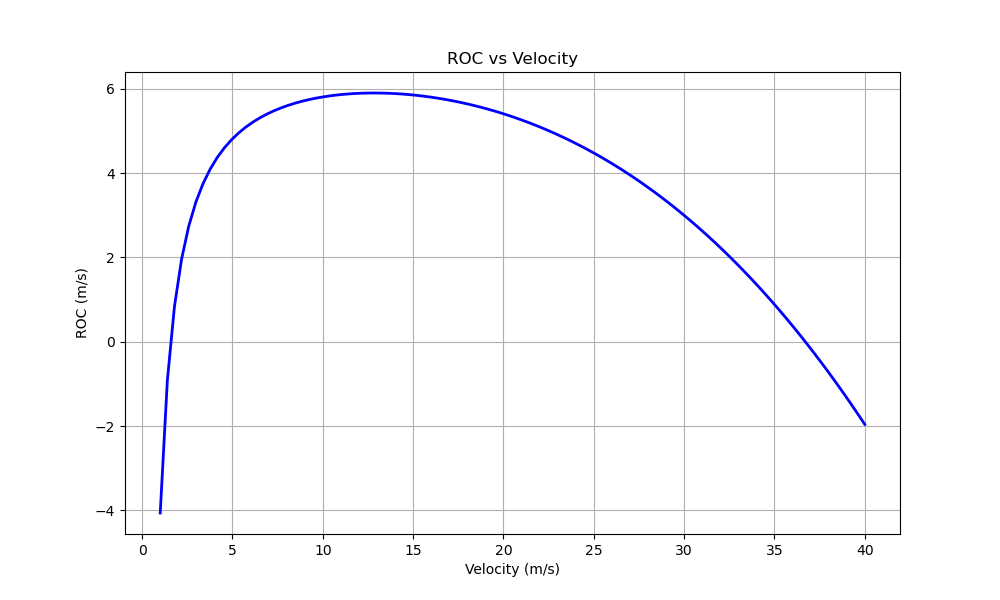
\includegraphics[width=\linewidth, height=0.72\textheight, keepaspectratio]{ROC_vs_Velocity.png}
    \caption{Rate of Climb vs. Airspeed}
  \end{figure}

\end{columns}
\end{frame}

% ========== SLIDE 12 — PERFORMANCE (2/2) ==========
\begin{frame}{Performance Parameters (2/2)}

\begin{columns}[T]

  \column{0.44\textwidth}
  \textbf{\color{navymain}Power Analysis:}
  \begin{figure}
    \centering
    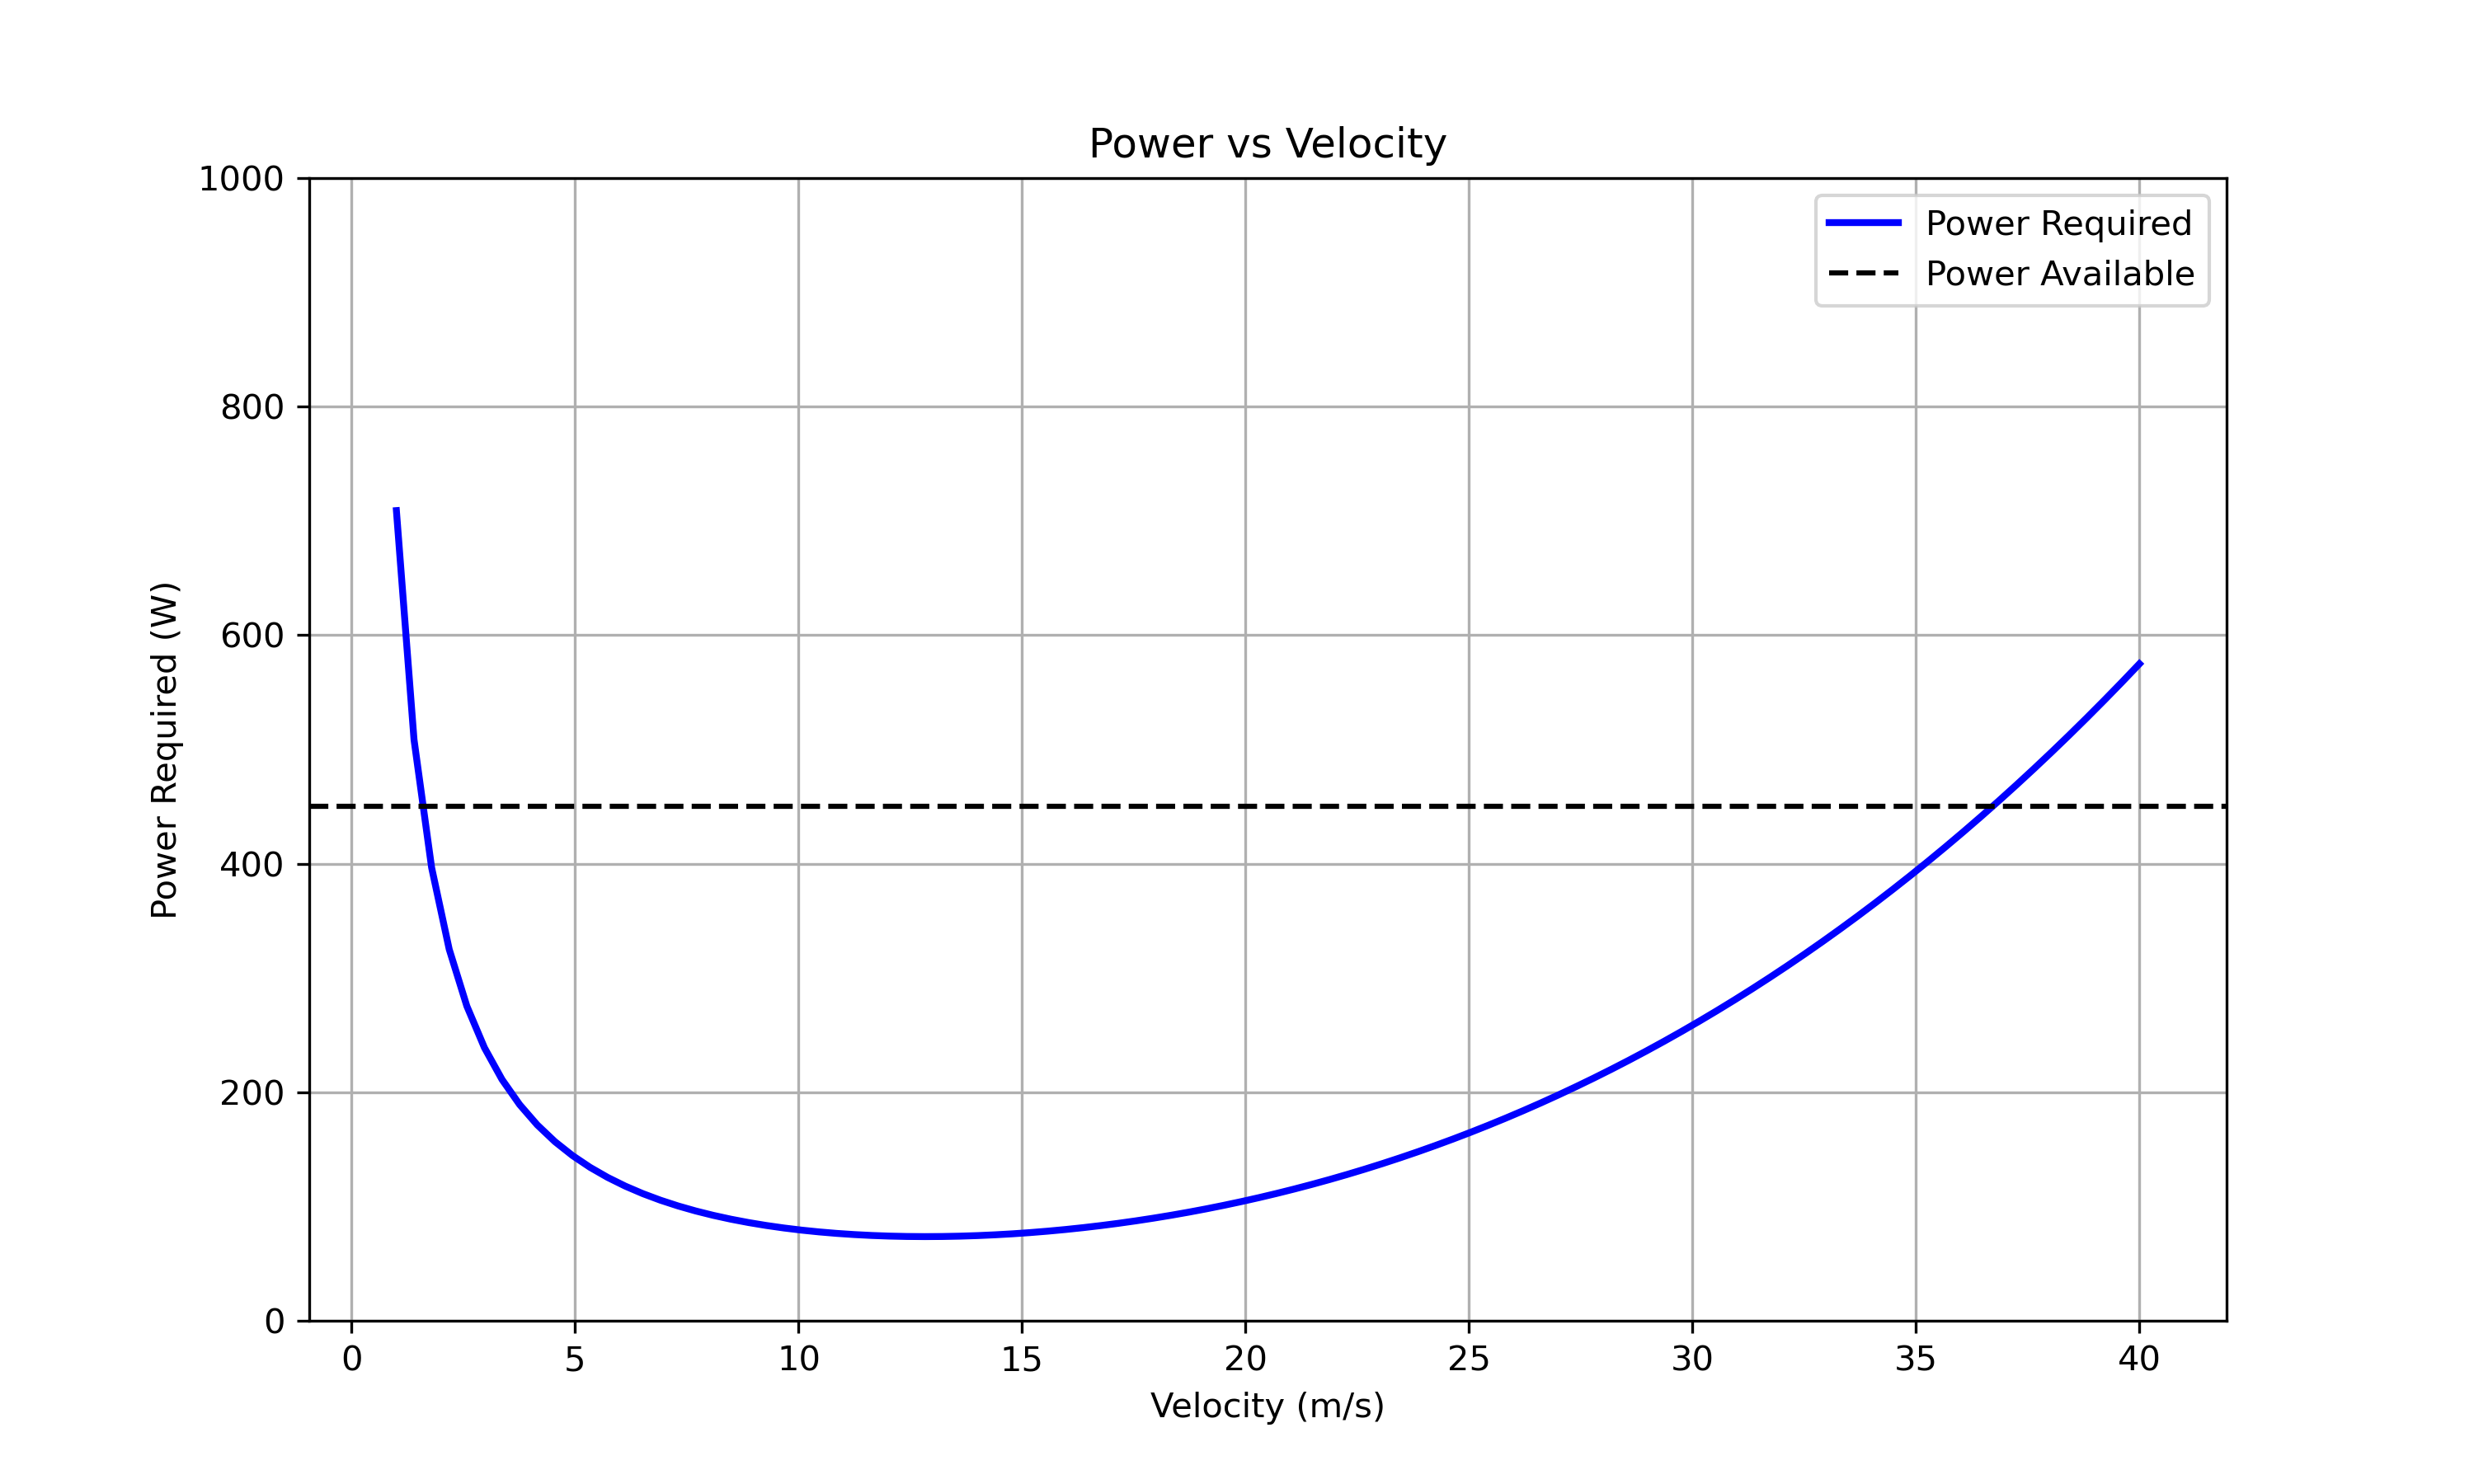
\includegraphics[width=\linewidth, height=0.38\textheight, keepaspectratio]{Power_vs_Velocity.png}
    \caption{Power Required vs. Airspeed}
  \end{figure}

  \vspace{0.1cm}
  \textbf{\color{navymain}STOL Performance:}
  \begin{itemize}\setlength\itemsep{2pt}
    \item Takeoff distance: \spec{$<\SI{150}{\meter}$}
    \item Liftoff velocity: \SI{13.6}{\meter\per\second}
    \item Landing distance: \spec{$<\SI{120}{\meter}$}
    \item Approach speed: \SI{15}{\meter\per\second}
  \end{itemize}

  \column{0.54\textwidth}
  \begin{figure}
    \centering
    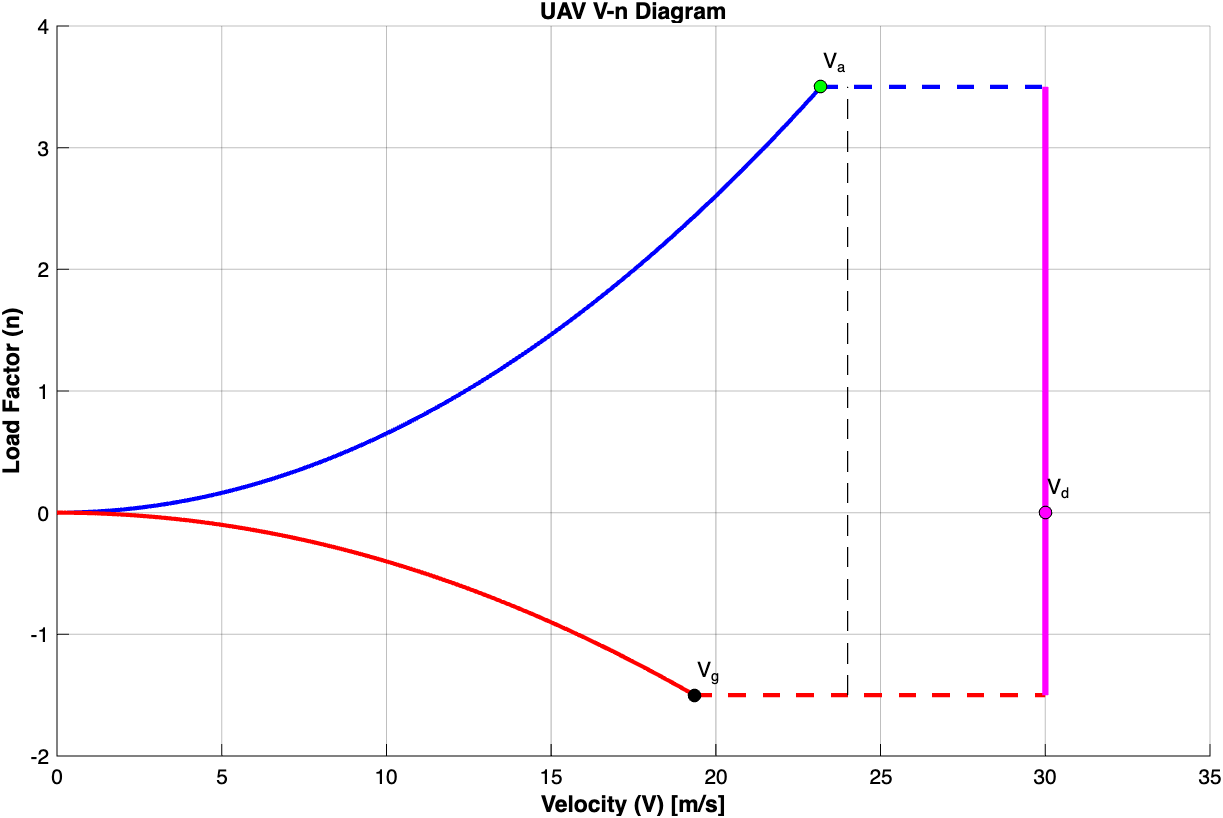
\includegraphics[width=\linewidth, height=0.50\textheight, keepaspectratio]{V_n_before_payload.png}
    \caption{UAV V-n Diagram (before payload drop)}
  \end{figure}

  \vspace{0.1cm}
  \begin{tabular}{@{}lcc@{}}
    \toprule
    \textbf{Param.} & \textbf{Req.} & \textbf{Achieved} \\
    \midrule
    Range (km)       & 80--100 & \spec{83.15} \\
    Endurance (h)    & 1--2    & \spec{2.08}  \\
    Cruise (m/s)     & 18--25  & \spec{18--22}\\
    Payload (kg)     & 1--2    & \spec{1.20}  \\
    \bottomrule
  \end{tabular}

\end{columns}
\end{frame}

% ========== SLIDE 13 — STABILITY (1/2) ==========
\begin{frame}{Stability Analysis (1/2) — Static}

\begin{columns}[T]

  \column{0.50\textwidth}
  \textbf{\color{navymain}Longitudinal Static Stability:}
  \begin{itemize}\setlength\itemsep{2pt}
    \item Static margin $K_n$: \spec{$\approx 14\%$ MAC}
    \item Neutral point: \SI{296}{\milli\meter} from nose
    \item CG location: \SI{264}{\milli\meter} from nose
    \item $C_{m_\alpha} = -0.487\;\mathrm{rad^{-1}}$ \textit{(stable)}
    \item $C_{m_0} = +0.0125$
  \end{itemize}

  \vspace{0.25cm}
  \textbf{\color{navymain}Lateral-Directional Static:}
  \begin{itemize}\setlength\itemsep{2pt}
    \item $C_{n_\beta} = +0.0838\;\mathrm{rad^{-1}}$ \textit{(dir. stable)}
    \item $C_{l_\beta} = -0.0111\;\mathrm{rad^{-1}}$ \textit{(dihedral eff.)}
    \item $C_{l_p}   = -0.659\;\mathrm{rad^{-1}}$  \textit{(roll damp.)}
  \end{itemize}

  \column{0.48\textwidth}
  \textbf{\color{navymain}Key Longitudinal Derivatives:}

  \vspace{0.2cm}
  \begin{tabular}{@{}lc@{}}
    \toprule
    \textbf{Derivative} & \textbf{Value} \\
    \midrule
    $C_{m_q}$  & $-14.94\;\mathrm{rad^{-1}}$ \\
    $C_{L_q}$  & $+5.66\;\mathrm{rad^{-1}}$  \\
    $C_{D_\alpha}$ & $+0.104\;\mathrm{rad^{-1}}$ \\
    $C_{L_M}$  & $+0.023$ \\
    \bottomrule
  \end{tabular}

  \vspace{0.4cm}
  \begin{block}{Stability Summary}
    \centering
    Statically \textbf{stable} in all axes.\\
    $14\%$ MAC static margin provides\\
    adequate pitch restoring moment.
  \end{block}

\end{columns}
\end{frame}

% ========== SLIDE 14 — STABILITY (2/2) ==========
\begin{frame}{Stability Analysis (2/2) — Dynamic Modes}

\begin{columns}[T]

  \column{0.40\textwidth}
  \textbf{\color{navymain}Longitudinal Modes:}
  \begin{itemize}\setlength\itemsep{2pt}
    \item \textbf{Short Period:}
      $\omega_n = \SI{7.53}{\radian\per\second}$,
      $\zeta = \spec{0.72}$ \textit{(well-damped)}
    \item \textbf{Phugoid:}
      $\omega_n = \SI{0.56}{\radian\per\second}$,
      $\zeta = 0.074$ \textit{(lightly damped)}
  \end{itemize}

  \vspace{0.3cm}
  \textbf{\color{navymain}Lateral-Directional Modes:}
  \begin{itemize}\setlength\itemsep{2pt}
    \item \textbf{Roll:}
      $\lambda_r = -14.0\;\mathrm{s^{-1}}$,
      $\tau_r = \SI{0.07}{\second}$ \textit{(fast)}
    \item \textbf{Dutch Roll:}
      $\omega_n = \SI{5.68}{\radian\per\second}$,
      $\zeta = 0.348$
    \item \textbf{Spiral:}
      $\lambda_s = +0.061\;\mathrm{s^{-1}}$
      \textit{(mildly unstable — typical)}
  \end{itemize}

  \column{0.58\textwidth}
  \begin{figure}
    \centering
    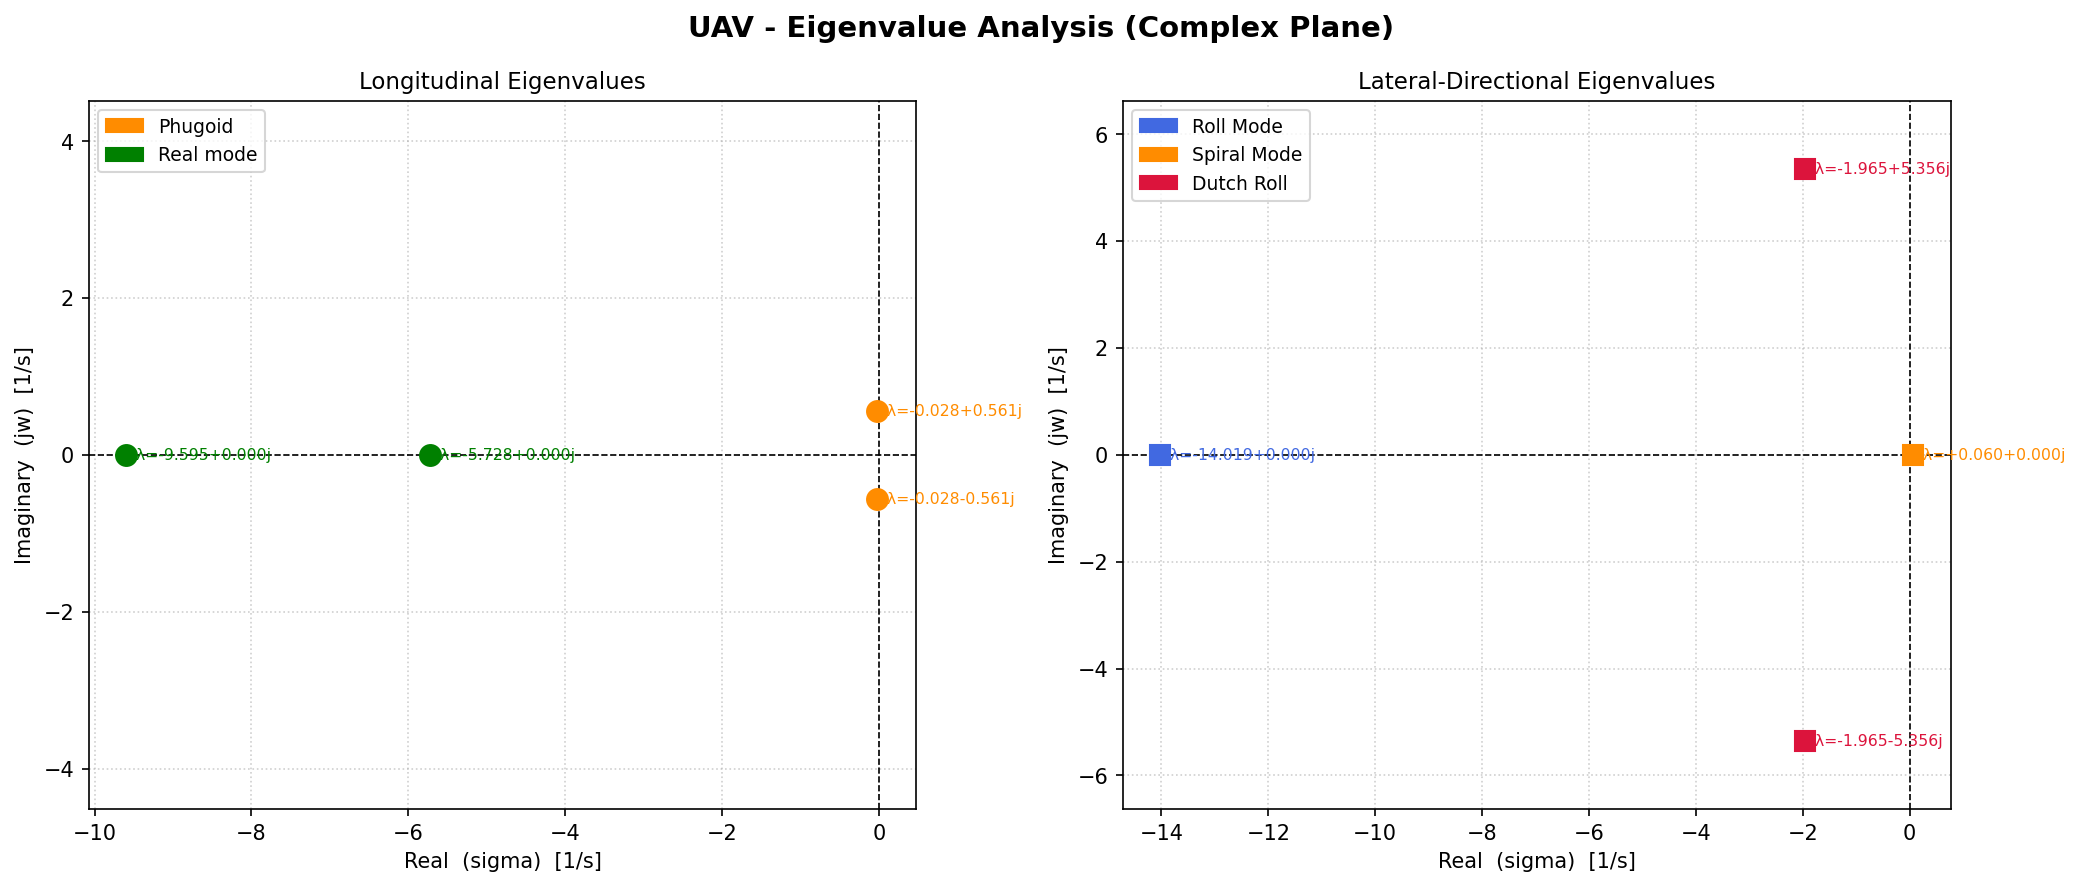
\includegraphics[width=\linewidth, height=0.78\textheight, keepaspectratio]{eigenvalue_plot.png}
    \caption{Eigenvalue Analysis — Longitudinal \& Lateral-Directional Modes}
  \end{figure}

\end{columns}
\end{frame}

% ========== SLIDE 15 — CAD MODEL (1/2) ==========
\begin{frame}{Detailed CAD Model (1/2) — Configuration}

\begin{columns}[T]

  \column{0.50\textwidth}
  \textbf{\color{navymain}Physical Configuration:}
  \begin{itemize}\setlength\itemsep{3pt}
    \item \textbf{Wing:} High-wing monoplane, rectangular
    \item \textbf{Propulsion:} Dual tractor motors on wing LE
    \item \textbf{Fuselage:} Modular with quick-swap payload bay
    \item \textbf{Empennage:} Conventional tail (T-config.)
    \item \textbf{Landing gear:} Tricycle configuration
    \item \textbf{Materials:} Carbon fibre spars, aluminium sheets
  \end{itemize}

  \vspace{0.35cm}
  \textbf{\color{navymain}Design Features:}
  \begin{itemize}\setlength\itemsep{2pt}
    \item Payload drop + parachute deployment
    \item Quick-release battery compartment
    \item Integrated avionics bay with telemetry
    \item Impact-absorbing landing gear for rough terrain
  \end{itemize}

  \column{0.48\textwidth}
  % Isometric CAD placeholder
  \textbf{\color{navymain}CAD Views:}
  \vspace{0.2cm}
  \begin{center}
    \colorbox{iceblue}{\parbox{0.88\linewidth}{%
      \centering\vspace{10pt}
      \textcolor{navymain}{\footnotesize\textbf{[Isometric View]}}
      \vspace{10pt}
    }}
    \vspace{0.1cm}

    \colorbox{iceblue}{\parbox{0.88\linewidth}{%
      \centering\vspace{8pt}
      \textcolor{navymain}{\footnotesize\textbf{[Top View]}}
      \vspace{8pt}
    }}
    \vspace{0.1cm}

    \colorbox{iceblue}{\parbox{0.88\linewidth}{%
      \centering\vspace{8pt}
      \textcolor{navymain}{\footnotesize\textbf{[Side View]}}
      \vspace{8pt}
    }}
  \end{center}

\end{columns}
\end{frame}

% ========== SLIDE 16 — CAD MODEL (2/2) ==========
\begin{frame}{Detailed CAD Model (2/2) — Component Integration}

\begin{columns}[T]

  \column{0.45\textwidth}
  \textbf{\color{navymain}Component Layout:}
  \begin{itemize}\setlength\itemsep{3pt}
    \item Flight controller \& GPS — nose bay
    \item Battery — forward fuselage (near nose)
    \item Payload compartment — at CG
    \item Motors — wing at 25\% chord LE
    \item 4$\times$ servo actuators
  \end{itemize}

  \vspace{0.5cm}
  \begin{block}{Design Philosophy}
    All removable/replaceable modules ease\\
    maintenance and \textbf{field deployment}.
  \end{block}

  \column{0.53\textwidth}
  % Front / 3-view CAD placeholder
  \begin{center}
    \colorbox{iceblue}{\parbox{0.92\linewidth}{%
      \centering\vspace{30pt}
      \textcolor{navymain}{\small\textbf{[Front View]}}
      \vspace{30pt}
    }}
    \vspace{0.2cm}
    \colorbox{iceblue}{\parbox{0.92\linewidth}{%
      \centering\vspace{28pt}
      \textcolor{navymain}{\small\textbf{[Three-View Drawing]}}
      \vspace{28pt}
    }}
  \end{center}

\end{columns}
\end{frame}

% ========== SLIDE 17 — REQUIREMENTS COMPLIANCE ==========
\begin{frame}{Requirements Compliance Summary}

\begin{center}
\begin{tabular}{@{}lccc@{}}
  \toprule
  \textbf{Requirement} & \textbf{Specification} & \textbf{Achieved} & \textbf{Status} \\
  \midrule
  Max wingspan      & \SI{2.00}{\meter}           & \spec{\SI{2.00}{\meter}}            & \textcolor{successgreen}{\checkmark} \\
  Payload capacity  & \SIrange{1}{2}{\kilo\gram}  & \spec{\SI{1.20}{\kilo\gram}}        & \textcolor{successgreen}{\checkmark} \\
  Operational radius& \SIrange{40}{50}{\kilo\meter}& \spec{\SI{41.6}{\kilo\meter}}      & \textcolor{successgreen}{\checkmark} \\
  Total range       & \SIrange{80}{100}{\kilo\meter}& \spec{\SI{83.15}{\kilo\meter}}    & \textcolor{successgreen}{\checkmark} \\
  Endurance         & \SIrange{1}{2}{\hour}       & \spec{2\,h\,5\,min}                 & \textcolor{successgreen}{\checkmark} \\
  Cruise speed      & \SIrange{18}{25}{\meter\per\second}& \spec{\SIrange{18}{22}{\meter\per\second}}& \textcolor{successgreen}{\checkmark} \\
  Takeoff (STOL)    & $<\SI{150}{\meter}$         & \spec{$<\SI{150}{\meter}$}          & \textcolor{successgreen}{\checkmark} \\
  Static stability  & Positive margin             & \spec{14\% MAC}                     & \textcolor{successgreen}{\checkmark} \\
  \bottomrule
\end{tabular}
\end{center}

\vspace{0.45cm}
\begin{center}

\begin{tikzpicture}
  \fill[navydeep, rounded corners=5pt] (0,0) rectangle (10.5,1.15);
  \node[text=white, font=\large\bfseries] at (5.25,0.575)
    {All Primary Mission Requirements Met \quad \textcolor{lightblue}{\checkmark}};
\end{tikzpicture}
\end{center}
\end{frame}

% ========== BACKUP SLIDE ==========
\appendix

\begin{frame}{Backup — Longitudinal Eigenvalue Plot}
  \begin{columns}[T]
    \column{0.40\textwidth}
    \textbf{\color{navymain}Longitudinal Modes (detail):}
    \begin{itemize}\setlength\itemsep{4pt}
      \item \textbf{Short Period:} \\
        $\lambda = -5.728 \pm 0j$ (real mode)
      \item \textbf{Phugoid:} \\
        $\lambda = -0.028 \pm 0.561j$
      \item Both modes lie in the \spec{left half-plane} — dynamically stable.
    \end{itemize}
    \column{0.58\textwidth}
    \begin{figure}
      \centering
      \includegraphics[width=\linewidth, height=0.75\textheight, keepaspectratio]%
        {Longitudinal_eigenvales.png}
      \caption{Longitudinal Eigenvalues}
    \end{figure}
  \end{columns}
\end{frame}

\begin{frame}{Backup — Lateral-Directional Eigenvalue Plot}
  \begin{columns}[T]
    \column{0.40\textwidth}
    \textbf{\color{navymain}Lateral-Directional Modes (detail):}
    \begin{itemize}\setlength\itemsep{4pt}
      \item \textbf{Roll:} $\lambda = -14.019$
      \item \textbf{Dutch Roll:} $\lambda = -1.965 \pm 5.356j$
      \item \textbf{Spiral:} $\lambda = +0.060$ \\
        \footnotesize(marginally unstable — standard for UAVs;\\
        correctable with autopilot)
    \end{itemize}
    \column{0.58\textwidth}
    \begin{figure}
      \centering
      \includegraphics[width=\linewidth, height=0.75\textheight, keepaspectratio]%
        {Lateral_eigenvalues.png}
      \caption{Lateral-Directional Eigenvalues}
    \end{figure}
  \end{columns}
\end{frame}

\end{document}
